%% ****** Start of file apstemplate.tex ****** %
%%
%%
%%   This file is part of the APS files in the REVTeX 4 distribution.
%%   Version 4.1r of REVTeX, August 2010
%%
%%
%%   Copyright (c) 2001, 2009, 2010 The American Physical Society.
%%
%%   See the REVTeX 4 README file for restrictions and more information.
%%
%
% This is a template for producing manuscripts for use with REVTEX 4.0
% Copy this file to another name and then work on that file.
% That way, you always have this original template file to use.
%
% Group addresses by affiliation; use superscriptaddress for long
% author lists, or if there are many overlapping affiliations.
% For Phys. Rev. appearance, change preprint to twocolumn.
% Choose pra, prb, prc, prd, pre, prl, prstab, prstper, or rmp for journal
%  Add 'draft' option to mark overfull boxes with black boxes
%  Add 'showpacs' option to make PACS codes appear
%  Add 'showkeys' option to make keywords appear
\documentclass[aps,pra,preprint,groupedaddress]{revtex4-1}
%\documentclass[aps,prl,preprint,superscriptaddress]{revtex4-1}
%\documentclass[aps,prl,reprint,groupedaddress]{revtex4-1}

\usepackage{graphicx}
\usepackage{amsmath}

% You should use BibTeX and apsrev.bst for references
% Choosing a journal automatically selects the correct APS
% BibTeX style file (bst file), so only uncomment the line
% below if necessary.
%\bibliographystyle{apsrev4-1}

\begin{document}

% Use the \preprint command to place your local institutional report
% number in the upper righthand corner of the title page in preprint mode.
% Multiple \preprint commands are allowed.
% Use the 'preprintnumbers' class option to override journal defaults
% to display numbers if necessary
%\preprint{}

%Title of paper
\title{Phase Dependent Ionization of Rydberg Atoms in Static Fields}

% repeat the \author .. \affiliation  etc. as needed
% \email, \thanks, \homepage, \altaffiliation all apply to the current
% author. Explanatory text should go in the []'s, actual e-mail
% address or url should go in the {}'s for \email and \homepage.
% Please use the appropriate macro foreach each type of information

% \affiliation command applies to all authors since the last
% \affiliation command. The \affiliation command should follow the
% other information
% \affiliation can be followed by \email, \homepage, \thanks as well.
\author{Eric Magnuson}
\email[]{edm5gb@virginia.edu}
\author{Tom Gallagher}
%\homepage[]{Your web page}
%\thanks{}
%\altaffiliation{}
\affiliation{University of Virginia, Department of Physics}

%Collaboration name if desired (requires use of superscriptaddress
%option in \documentclass). \noaffiliation is required (may also be
%used with the \author command).
%\collaboration can be followed by \email, \homepage, \thanks as well.
%\collaboration{}
%\noaffiliation

\date{\today}

\begin{abstract}
Pump-probe schemes using high frequency pulsed light synchronous to strong field low frequency fields are a prolific tool for probing atomic, molecular and surface electron dynamics. We realize one such system in Rydberg states of Li using an 819-nm excitation laser amplutde modulated synchronously to a 15.9-GHz microwave field. We show that when the modulation is at the same frequency of the microwave field, phase dependent ionization is only observed in the presence of static fields. Our results are well described by a computational model. Analysis of this model shows the importance of multiple classical electron orbits.
\end{abstract}

% insert suggested PACS numbers in braces on next line
\pacs{}
% insert suggested keywords - APS authors don't need to do this
%\keywords{}

%\maketitle must follow title, authors, abstract, \pacs, and \keywords
\maketitle

% body of paper here - Use proper section commands
% References should be done using the \cite, \ref, and \label commands
\section{\label{intro}Introduction}
% Put \label in argument of \section for cross-referencing
%\section{\label{}}
%\subsection{}
%\subsubsection{}

\section{Background}
\label{sec:back}

\section{Experimental Methods}
\label{sec:exp}

In this experiment, Li atoms in a columated thermal beam are optically excited to high lying Rydberg or continuum states along the path $2s \xrightarrow{\text{671-nm}} 2p \xrightarrow{\text{610-nm}} 3d \xrightarrow{\text{819-nm}} nf, \epsilon f$. These optical beams intersect at a right angle forming a rectangular 1 mm$^3$ excitation region. This region is at an anti-node of a 15.9 GHz Fabry-Perot microwave cavity. The 1 mm$^3$ region is much smaller than the extent of the microwave antinode, allowing us to consider the microwave field constant across the region. The interaction region is enclosed on top, bottom and two sides by aluminum plates. Combined with the two Fabry-Perot mirrors, this forms a 10-cm cubic enclosure. Bias voltages can be applied independently to each plate and mirror to control static fields in the interaction region.

The microwave cavity is allowed to load for 240 ns before the first laser pulse, and the microwave input is shut off 20 ns after the last laser pulse allowing the cavity to empty. Synchronous with the MW power envelope, a static field pulse is applied to the top and bottom aluminum plates to produce a vertical static field in the interaction region. The 610-nm and 671-nm lasers are pulsed synchronously for 20 ns, after which the 819-nm laser is pulsed with a square envelope for 20 ns. One microsecond after the last laser pulse, we field ionize surviving Rydberg states within 100 GHz of the ionization limit by applying a negative voltage pulse to an aluminum plate below the interaction region. Ionized electrons are pushed into a microchannel plate (MCP) assembly which produces a voltage pulse proportional to the number of electrons detected. This pulse is integrated through a boxcar integrator and recorded.

\begin{figure}
	\includegraphics[width=0.5\textwidth]{fields}
	\caption{Temporal view of the microwave field (top) phase-locked with the amplitude modulated laser intensity (bottom). The peak laser intensity occurs at the phase $\omega_0 t$ of the microwave field, and can be adjusted by an optical delay line.}
	\label{fig:AMLaser}
\end{figure}

Probing phase dependence in this experiment is achieved by synchronizing the amplitude modulation of the 819-nm laser to a microwave field in the cavity, as shown in Fig.~\ref{fig:AMLaser}. The laser field can be described by an envelope modulating a fundamental frequency:
\begin{equation}
E_{opt}(t) = E_o \sin{(\omega_o t)} \cos{(\omega(t-t_0))}
\end{equation}
Using an optical delay line, the phase of the modulation envelope of the 819-nm laser can be delayed relative to phase of the microwave field. This modulation is proportional to the excitation-rate to a Rydberg or continuum state, so delaying the modulation envelope is equivalent to changing the phase $\omega t_0$ of the microwave field at which excitation occurs.

\subsection{Dye Lasers}
\label{sec:dye}

We use two dye lasers at 670-nm and 610-nm to drive the $2s \rightarrow 2p$ and $2p \rightarrow 3d$ transitions, respectively. These dye lasers are pumped by a Quantronix Darwin Nd:YLF. The pump laser produces 30-W, approximately 100-ns FWHM pulses at a 1-kHz repetition rate. Using a Pockels cell (PC) and polarizing beam splitter (PBS), the rising edge of the pulse is picked off and split equally between to the 670-nm and 610-nm lasers. A second PC and PBS directs a 20-ns slice from the peak of the pump pulse to a dye amplifier for the 819-nm laser. The long trailing edge of the pump pulse is dumped.

The 670-nm dye laser uses a Littman-style cavity and LDS-698 laser dye dissolved in Ethanol as a lasing medium. The 610-nm uses a H{\"a}nch style cavity with Rhodamine-610 laser dye dissolved in Ethanol. Both lasers have an approximate FWHM of 10-GHz. To minimize unintended ionization from the $3d$ state, both lasers are attenuated to 2 $\mu J$ pulses before being directed to the vacuum chamber.

\subsection{Amplitude Modulated 819-nm Laser}
\label{sec:ampmod}

\begin{figure}
	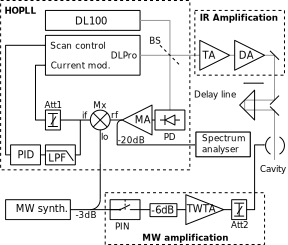
\includegraphics[width=0.5\textwidth]{beatexp}
	\caption{Schematic showing how the amplitude modulated laser is produced, locked to the microwave frequency, and how both the laser and microwave fields are delivered to the interaction region. The AM IR laser is generated by overlapping the DL-Pro and DL-100 laser beams on a beamsplitter (BS). One output is amplified and sent to the interaction region. The microwave field is generated by a synthesizer, formed into pulses by the PIN switch and amplified by the Traveling Wave Tube Amplifier (TWTA) before injection into the microwave cavity. The locking of the IR intensity envelope to the microwave field is performed by the Heterodyne Optical Phase Locked Loop (HOPPL).}
	\label{fig:pll}
\end{figure}

Fig.~\ref{fig:pll} shows how the amplitude modulated laser and microwave fields are produced and delivered to the interaction region, and how they are locked in a phase locked loop. The 819-nm laser is produced from two external-cavity diode lasers, a Toptica DL-100 and DL-Pro. They are tuned so that they are separated by the microwave frequency, and overlapped on a 50:50 beamsplitter. This overlapping produces a beat-note in the laser intensity at the microwave frequency. One output from the beamsplitter is directed to a high speed photodetector that can detect the beat note and deliver the signal to the phase-locked-loop. The second output from the beamsplitter is directed through an amplification chain and to the interaction region.

The amplitude modulation of the laser is locked at the microwave frequency with a phase-locked-loop (PLL). The locking is driven by a "fast" feedback to the current input of the DL-Pro, and a "slow" feedback to the scan input. To produce an error signal, the amplitude modulation is detected after the 50:50 beamsplitter by a fast photodiode. The DC signal is filtered out, leaving only the AC component. This is amplified and mixed with the microwave source to produce an error signal. The error signal is passed through a variable attenuator and then connected to the Current input of the Toptica DL-100. This achieves a lock between the laser ampltude modulation frequency and the microwave field that lasts for several minutes.

To achieve longer lock times on the order of hours, we use a Toptica PID-110 to drive the scan input of the DL-Pro. The "fast" current lock is primarily lost due to the lasers drifting past the range that the current input can correct. Low-frequency components of the error signal are processed through a PID and fed to the Scan input. This corrects long term drifts in the amplitude modulation frequency, leaving only high-frequency errors for the "fast" loop to correct.

The second output of the 50:50 beamsplitter produces 30 mW of aplitude modulated light. This is passed through a tapered amplifier and a dye amplifier. The Toptica Tapered Amplifier increases the continuous beam power to 800 mW. The dye amplifier is pumped by a 20-ns square pulse picked from the peak of the Nd:YLF laser pulse. We use LDS-819 dissolved in Ethanol as the amplfication medium. This outputs a 20-ns long, 6 $\mu$W pulse of amplitude modulated 819-nm light.

\subsection{\label{cavity} Microwave Apparatus}

A Hittite HMC T-2100 synthesizer tuned to the 15.9-GHz resonance of the microwave cavity is used as our microwave source. The Hittite produces 9 dBm, and a splitter diverts half of the power to the microwave mixer to generate the error signal for the PLL. The other half of the signal is formed into 300-ns pulses by a microwave switch, and then amplified by a Hughes 8020H04F traveling-wave-tube-amplifier (TWTA). Between the TWTA and the cavity, there is a 0 to 50 dBm variable attenuator allowing us to control the intensity of the pulse incident on the microwave cavity.

The microwave cavity is a Fabry-Perot cavity composed to two brass spherical mirrors. These mirrors have a radius of curvature of 10 cm and are 10.2 cm in diameter, with an on axis separation of 7.83 cm. The 15.9 GHz resonance is the TEM$_{008}$ mode of the cavity, with a quality of 3600 \emph{CAVITY QUALITY}. We are able to determine the field inside the cavity to \emph{15\%}.

\subsection{\label{fields} Static Fields}

This experiment depends on the detection of long lived Rydberg states close to the ionization limit. To prevent these states from ionizing before detection, we must minimize the persistent static field in the interaction region. We accomplish this by surrounding the interaction region on two sides with the brass microwave cavity mirrors, and on the remaining two sides, top, and bottom with polished aluminum plates. A voltage can be applied independently to each plate or mirror, allowing us to compensate persistent static fields in every direction. We measure the depressed ionization limit (DIL) to minimize stray fields and estimate the residual persistent static field. In this manner, we determine the remaining persistent static field to have a magnitude of 1.5 mV / cm. \emph{ADD REFERENCE}.

To observe phase dependent ionization, we need to apply a pulsed vertical static field to the interaction region during excitation of Rydberg states. This is done using a two-channel arbitrary waveform generator (AWG) to apply 300-ns square pulses of opposite magnitudes to the top and bottom bias plates. This square pulse is synchronous with the microwave pulse, the leading edge arriving 240-ns before the first laser pulse and the trailing edge arriving 20-ns after the end of the 819-nm laser pulse. Turning off the applied static field minimizes the static field ionization of the high-lying states we wish to observe. 1 $\mu s$ after the final laser pulse, the same AWG applies a voltage to the bottom plate to produce a -0.65 V / cm ionization field, ionizing high-lying states and pushing ionized electrons toward the MCP stack.

\section{\label{results}Results}

\begin{figure}
	\includegraphics[width=0.5\textwidth]{PhaseDelay}
	\caption{Observed Rdyberg signal as the phase delay is scanned. When no static field is applied, there is no observed phase modulation at the microwave frequency. When a 14 mV/cm static field is applied, there is a clear phase dependence in the Rydberg signal. For this measurement, the central frequency of the excitation laser is tuned to 14 GHz below the depressed ionization limit (DIL), and the microwave field inside the cavity is 4 V/cm.}
	\label{fig:PhaseDelay}
\end{figure}

Fig.~\ref{fig:PhaseDelay} shows that, when the laser intensity is modulated at the same frequency as the microwave field, a phase dependent ionization can only be observed when a static field is present during excitation. The central frequency of the excitation laser is tuned to 14-GHz below the DIL, in the presence of a 4 V/cm microwave field \emph{CALIBRATION}. The relative phase delay is scanned while measuring the Rydberg signal. Two such scans are completed, one without applying a pulsed static field, one while applying a 14 mV/cm pulsed static field. It is clear that adding the static field allows us to observe phase dependence. This confirms the prediction made by our model, that phase dependent ionization can only be observed at the microwave field frequency when a static field is applied to lift the vertical symmetry of the system.

We quantify these observations by fitting the signal vs. delay to a sinusoidal model:
\begin{equation}
S = A \cos{[\omega t - \phi_0]} + S_0
\end{equation}
The model frequency is fixed at $\omega = 2\pi / f_{mw}$, while the amplitude (A), phase offset ($\phi_0$) and mean signal ($S_0$) are used as fit parameters. To further explore this phenomena, we record how these fit parameters change as we vary the applied static field for three tunings of the excitation laser central frequency: 2-GHz above, and 14 and 30 GHz below the DIL.

\begin{figure}
	\includegraphics[width=0.5\textwidth]{ModvsField}
	\caption{Mean signal ($S_0$) and peak-to-peak modulation ($2\cdot A$) against applied pulsed static field for excitation laser central frequencies of +2 GHz, -14 GHz, and -30 GHz relative to the DIL. A negative peak-to-peak amplitude indicates a phase modulation with a phase shift ($\phi_0$) of $\pi$.}
	\label{fig:ModvsField}
	\end{figure}

Fig.~\ref{fig:ModvsField} shows plots of both peak-to-peak phase dependence in the signal ($2\cdot A$) as well as mean signal ($S_0$) as a function of applied pulsed static field at 3 different laser tunings. For all three laser tunings, the mean signal behaves as expected. The signal is largest when there is no static field applied, and the high lying states we detect are longer lived. As the magnitude of the applied static field increases, mean signal monotonously decreases as the high lying states are more likely to ionize. As would be expected, the further below the DIL the central frequency of the excitation laser is tuned, the more slowly $S_0$ drops off with field.

The observed behavior of the peak-to-peak modulation is more complex. In Fig.~\ref{fig:ModvsField} \emph{(A) LABEL SUBPLOTS} showing observations with a laser tuning 2 GHz above the DIL, the peak-to-peak modulation behaves in an expected way. At zero static field, we can observe no phase dependence for symmetry reasons. However, as the static field magnitude is increased phase dependence quickly emerges. Then, as the total signal approaches zero, so does the peak-to-peak modulation. In these figures, the fit parameter $\phi_0$ is restricted to a range of 0-$\pi$, shifts outside of this range are accounted for with a negative amplitude $A$. Because the applied static field is the only parameter lifting the vertical symmetry, applying an inverse static field produces inverse phase dependence. This shows in the peak-to-peak modulations at opposite applied static fields being approximately equal and opposite.

In the two figures at 14 GHz and 30 GHz below the DIL, the behavior is more complex. First, at low static fields, the peak to peak modulation is inverted relative to observations made at 2 GHz above the limit. As the applied static field increases, the peak-to-peak modulation increases to a maximum, but then decreases to zero and changes sign (equivalent to a phase shift of $\pi$). After this zero-crossing, the peak-to-peak modulation then increases to a maximum, and slowly decreases to zero as in the above-the-limit observation. From the two scans below the DIL, it's clear that the further below the DIL the central frequency of the laser is tuned to, the larger the static field applied before this zero crossing is reached. Further, the scan at 30 GHz below the DIL shows there may be an "activation static field" below which phase dependence cannot be observed.

The behavior of the mean signal for all laser tunings, as well as the peak-to-peak modulation in the +2 GHz observation are explained by the fundamentals of our model. However, it is not clear why at small applied static fields, the peak-to-peak modulation below the ionization limit is of opposite sign compared to observations above the ionization limit. It is also not immediately obvious why the modulation approaches zero and then changes sign at a particular static field. To investigate these phenomena, we produced a computational model.

\section{Computational Model}
\label{sec:comp}

We modeled our system as a classical electron excited to a particular energy and angular momentum by the excitation laser, moving in the presence of the core Coulomb potential as well as the applied static and microwave fields. The electron moves in the system for 80 ns after excitation, during which time the static field has turned off, and the microwave cavity has been allowed to ring down. The Rydberg states we are investigating are long-lived, so after the static and microwave fields are no longer present the electron will not be disturbed from whatever final state it has arrived at.

In atomic units, the equations of motion executed by the simulation are:
\begin{equation}
\ddot{\vec{r}} = -\frac{1}{r^2} \cdot \hat{r} - \Theta_{st}(t) \vec{E}_{st} - \Phi_{mw}(t) \vec{E}_{mw} \sin{(\omega t + \phi_0)},
\end{equation}
where $\Phi_{mw}(t)$ and $\Theta_{st}(t)$ are the envelopes of the microwave and static fields, respectively.
\begin{align}
\Phi_{mw}(t<t_{off}) & = 1 & \quad & \Theta_{st}(t<t_{off}) & = 1 \\
\Phi_{mw}(t \geq t_{off}) & = e^{-(t-t_{off})/\tau} & \quad & \Theta_{st}(t \geq t_{off}) & = 0
\end{align}
To match the conditions of our experiment, the ring-down time of the microwave cavity is $\tau = 10 ns$, and the time at which the fields are turned off are $t_{off} = 20 ns$. The microwave frequency is $\omega = 2\pi \cdot 15.9 GHz$ and the microwave field is set to $\vec{E}_{mw} = 4 V/cm \hat{z}$. The pulsed electric field $\vec{E}_{st}$ is always along the $\hat{z}$ axis, and simulations are executed at a variety of magnitudes. $\phi_0$ represents the initial phase of the microwave field at which the electron is excited.

The initial conditions of the electron can be set to the classical equivalent of an electron excited to an orbit with a particular initial kinetic energy and angular momentum. Further, because the electron is excited from the much smaller $3D$ state, the initial position is chosen to be the point of closest approach in the classical orbit. There is, however, no classical analog to an $m_l = 0$ state to dictate whether an orbit confined to the $x-z$ plane aught to have it's initial angular momentum vector pointed in the $+/- \hat{y}$ direction. As such, for each set of parameters, both initial conditions are considered. Finally, because our excitation laser frequency is much faster than the microwave frequency, we consider both cases where the the elliptical orbits are elongated in the $+ \hat{z}$ and $-\hat{z}$ directions, corresponding to initial Laplace-Runge-Lenz (LRL) vectors in the $+\hat{z}$ and $-\hat{z}$ directions. In total, for each particular $\phi_0$ and $\vec{E}_{st}$, four separate cases are considered.

\begin{figure}
	\includegraphics[width=0.5\textwidth]{14}
	\caption{\emph{LABEL (A)(B)(C).} The analysis converting a set of simulation runs at 200 phases $\phi_0$ between 0 and 2$\pi$, with a pulsed static field of 14 V/cm, a microwave field of 4 V/cm, and an excitation energy of 20 GHz below the ionization limit. For each $\phi_0$, the simulation is run for initial angular momentum in the $+\hat{y}$ and $-\hat{y}$ directions, and initial LRL vectors in the $+\hat{z}$ and $-\hat{z}$ directions. (A) shows the final total orbital energy after the system has evolved for 80 ns. In (B), these final energies are sorted into $E_f\geq 0$ and $E_f<0$ corresponding to ionized and bound states, respectively. (C) shows the results of convolving the results from (B) with the intensity profile of the amplitude modulation. The combined signal from the "up" and "down"-hill electrons is observed experimentally.}
	\label{fig:ModEval}
\end{figure}

The process for simulating an experimental result for a particular choice of $\vec{E}_{st} = + 14 mV/cm \hat{z}$ and an initial energy corresponding to 20 GHz below the ionization limit is shown in Fig.~\ref{fig:ModEval}. We iterate the initial excitation phase $\phi_0$ over 200 points between 0 and $2\pi$, corresponding to portions of the electron wave-packet excited at different phases of the microwave field. The system is allowed to evolve for 80 ns, at which point we extract the final orbital energy $E_f$ of the electron. If $E_f \geq 0$ we consider the electron ionized and assume we will not detect it. If $E_f < 0$, we consider the electron bound and assume it will be stable until it is field ionized and detected 1 $\mu s$ later. This set of final states is convolved with the intensity modulation envelope of the excitation laser to produce the expected phase-dependent Rydberg signal.
\begin{equation}
S(\phi) = \frac{1}{4n} \sum_{i=0}^{n} F(\phi\prime_i) \cdot \cos{^2(\phi - \phi\prime_i)}
\end{equation}

\begin{figure}
\includegraphics[width=0.5\textwidth]{fields0}
\caption{Phase dependent Rydberg signal produced by our computational model.}
\label{fig:SimMod}
\end{figure}

Fig.~\ref{fig:SimMod} shows the results of our computational model with an initial electron energy of -20 GHz, a 4 V/cm microwave field, at different pulsed fields. This model provides insight into how phase dependence emerges as the applied field is increased. At zero field, it is clear that the electrons launched "uphill", along the electric field, produce a signal exactly $\pi$ out of phase with electrons launched "downhill", opposite the electric field direction. The combined signal from these two groups then produces a flat detected signal. However, when a small 14 mV/cm static field is applied, the uphill and downhill signals differentiate. As should be expected, the downhill electrons have the same signal phase, but the mean value of the signal is suppressed. This corresponds to a depressed potential in the downhill direction causing fewer electrons to remain bound. Something interesting, however, happens to the uphill electrons at low fields. The phase that takes energy from electrons to produce more bound states in zero-field leads to more ionization in small fields. Meanwhile, the phase that adds energy to the electron is more likely to produce bound states. Examination of orbits in our model shows that this is do to the uphill potential catching electrons with increased energy in long orbits that do not return to the ion core before the microwave field dies off, and are therefore unlikely to ionize. Uphill electrons launched at phases that lose energy, conversely, are put into deeper, fast orbits that pass near the core many times while the microwave fields are strong, providing many opportunities to gain energy from the microwave field and ionize. Combined, these up- and downhill electron signals produce a clear combined phase dependent Rydberg signal.

Just as is shown in our experimental data, the phase of the total signal produced by our model shifts by $\pi$ at large pulsed fields. From looking at up- and downhill electron contributions, there are two important causes for this phase inversion. First, the downhill electron signal is almost completely suppressed at large static fields. This is sensible, at some point the classical turning point in the core + static potential is too depressed to trap any downhill electrons. The combined signal is then almost entirely due to electrons launched uphill. Investigating the electron orbits in our model shows the uphill signal phase shift is due to the long orbits present at smaller fields disappearing. Instead, electrons both gaining and losing energy in the microwave field end up in orbits that return to the core many times, allowing for ionization. The result is that more deeply bound electrons are further from ionization and are less likely to ionize. Our classical computational model, accounting for multiple orbits of excited Rydberg electrons, can account for both the onset of phase dependence with applied pulsed static field, and the inversion of phase dependence observed at large static fields.

\section{Discussion}
\label{sec:disc}

\section{Conclusions}
\label{sec:conc}

% If in two-column mode, this environment will change to single-column
% format so that long equations can be displayed. Use
% sparingly.
%\begin{widetext}
% put long equation here
%\end{widetext}

% figures should be put into the text as floats.
% Use the graphics or graphicx packages (distributed with LaTeX2e)
% and the \includegraphics macro defined in those packages.
% See the LaTeX Graphics Companion by Michel Goosens, Sebastian Rahtz,
% and Frank Mittelbach for instance.
%
% Here is an example of the general form of a figure:
% Fill in the caption in the braces of the \caption{} command. Put the label
% that you will use with \ref{} command in the braces of the \label{} command.
% Use the figure* environment if the figure should span across the
% entire page. There is no need to do explicit centering.

% \begin{figure}
% \includegraphics{}%
% \caption{\label{}}
% \end{figure}

% Surround figure environment with turnpage environment for landscape
% figure
% \begin{turnpage}
% \begin{figure}
% \includegraphics{}%
% \caption{\label{}}
% \end{figure}
% \end{turnpage}

% tables should appear as floats within the text
%
% Here is an example of the general form of a table:
% Fill in the caption in the braces of the \caption{} command. Put the label
% that you will use with \ref{} command in the braces of the \label{} command.
% Insert the column specifiers (l, r, c, d, etc.) in the empty braces of the
% \begin{tabular}{} command.
% The ruledtabular enviroment adds doubled rules to table and sets a
% reasonable default table settings.
% Use the table* environment to get a full-width table in two-column
% Add \usepackage{longtable} and the longtable (or longtable*}
% environment for nicely formatted long tables. Or use the the [H]
% placement option to break a long table (with less control than 
% in longtable).
% \begin{table}%[H] add [H] placement to break table across pages
% \caption{\label{}}
% \begin{ruledtabular}
% \begin{tabular}{}
% Lines of table here ending with \\
% \end{tabular}
% \end{ruledtabular}
% \end{table}

% Surround table environment with turnpage environment for landscape
% table
% \begin{turnpage}
% \begin{table}
% \caption{\label{}}
% \begin{ruledtabular}
% \begin{tabular}{}
% \end{tabular}
% \end{ruledtabular}
% \end{table}
% \end{turnpage}

% Specify following sections are appendices. Use \appendix* if there
% only one appendix.
%\appendix
%\section{}

% If you have acknowledgments, this puts in the proper section head.
%\begin{acknowledgments}
% put your acknowledgments here.
%\end{acknowledgments}

% Create the reference section using BibTeX:
\bibliography{basename of .bib file}

\end{document}
%
% ****** End of file apstemplate.tex ******

